\chapter{Lecture \thechapter{} of 11/03/2026}

We ask ourselfs what happens if $f$ is convex and we add some regularity hypotesis. We first remark that if $f$ is differentiable at $c$, near this point, the function looks like an hyperplane. The intuition is: function must be always above its tangent hyperplane.

\begin{proposition}
    
    Let $C \seq \Rn$ be convex, $A \seq \Rn$ open s.t. $C \seq A$. Let $f: A \to \R$ convex and differentiable. Then 

    \begin{enumerate}
        \item[$i)$] $f$ is convex on $C \iff f(z) \ge f(x) + \langle \nabla f(x), z - x \rangle$ for all $x,z \in C$
        \item[$ii)$] $f$ is strictly convex over $C \iff f(z) > f(x) + \langle \nabla f(x), z-x \rangle$ for all $x,z \in C$ s.t. $x \neq z$
    \end{enumerate}

\end{proposition}

\begin{proof}
    
    Let $f$ be convex on $C$. Let $x,z \in C$. Observe that 

    \[ \lim_{h \to 0^+} \frac{f(x + h(z-x)) - f(x)}{h} = \frac{\partial}{\partial h} f(x + h(z-x))|_{h=0} = \nabla f(x) \cdot (z-x). \]

    Then

    \begin{align*}
        f(x) + \langle \nabla f(x), z - x \rangle &= f(x) + \lim_{h \to 0^+} \frac{f(x + h(z-x)) - f(x)}{h} \\
        &= \lim_{h \to 0} \frac{hf(x) - f(x) + f(hz + (1-h)x)}{h} \\
        &\le \lim_{h \to 0} \frac{-(1-h)f(x) + hf(z) - (1-h)f(x)}{x} \\
        &= \lim_{h \to 0} f(z) = f(z).
    \end{align*}

    Let now $\alpha \in [0,1]$, $x,y \in C$, $z = \cc$. 

    \begin{align*}
        f(x) &\ge f(z) + \langle \nabla f(z) , x-z \rangle \cdot \alpha \\
        f(y) &\ge f(z) + \langle \nabla f(z), y-z \rangle \cdot (1-\alpha)
    \end{align*}

    Take the sum of the above quantities, then 

    \[ \alpha f(x) + (1-\alpha)f(y) \ge \alpha f(z) + (1-\alpha)f(z) + \alpha \langle \nabla f(z) , x-z \rangle + (1-\alpha) \langle \nabla f(z), y-z \rangle \]

    hence, by linearity of the scalar product, 

    \[ \alpha f(x) + (1-\alpha)f(y) \ge f(z) + \langle \nabla f(z), \alpha x + (1-\alpha)y - z \rangle. \]

    Hence, $f$ is convex.

    For the strict convexity, we repeat the same process with the strict inequality.

\end{proof}

If at some point $x^*$ we have $\langle \nabla f(x^*), z-x^*\rangle \ge 0$ for all $z$, then $x^*$ is a minimum point. This is also a necesary condition: assume $x^*$ minumum point for $f$ over $C$ and, by contraddiction, thath there exists $z \in C$ s.t. $\langle \nabla f(x^*), z-x^* \rangle < 0$, but then 

\[ \frac{\partial}{\partial h} f(x^* + h(z - x^*))|_{h=0} = \langle \nabla f(x^*), z-x^*\rangle < 0 \]

so $f$ decreases in the direction $z - x^*$, which contrdaddicts the fact that $x^*$ is a minimum.

We summarize this fact in the following proposition, which proof what we just did.

\begin{proposition}
    
    Let $C \seq \Rn$ be convex, $f: \Rn \to \R$ be differentiable on a convex open set $A \seq C$. Then a point $x^* \in C$ is a minimum for $f$ if and only if 

    \[ \langle \nabla f(x^*), z-x^*\rangle \ge 0 \quad \forall z \in C. \]

\end{proposition}

\begin{theorem}[Projection theorem]

    Let $C$ be a nonempty convex closed sunset of $\Rn$, $z \in \Rn$. Then there exists a unique vector $x^* \in C$ (the projection of $z$ on $C$) that minimizes the function $f(x) = \norm{x- z}$ over $C$. 

    Furthermore, the point $x^*$ is the projection of $z$ onto $C$ if and only if 

    \[ \langle z - x^*, x - x^* \rangle \le 0 \quad \forall x \in C. \]
    
\end{theorem}

\begin{proof}
    
    Optimizing the function $f(x) = \norm{z-x}$ is the same as optimizing the funciton $f(x) = \frac12 \norm{z-x}^2$. Then $f$ is now differentiable, and $\nabla f(x) = z-x$. 

    \begin{align*}
        x^* \text{ is minimum }&\iff \langle \nabla f(x^*), x - x^* \rangle \ge 0 \quad \forall x \in C \\
        &\iff \langle -x^* + z, x - x^* \rangle \le 0.
    \end{align*}

    Does such an $x^*$ exists? We observe that 

    \[ \min_{x \in C} f(x) = \min_{x \in C \cap \set{y : \norm{y-z} \le \norm{z-w}}, \, w \in C} f(x). \]

    We notice that we are optimizing a continous function on a closed set, as we are optimizing on $C \cap \overline{B(z,\norm{z-w})}$, so, by Weierstrass there exists a minimum. This is also unique, indeed, let $x^*_1,x^*_2$ be two minima, then 

    \begin{align*}
        \langle z - x^*_1, x^*_2-x^*1 \rangle &\le 0 \quad \forall z \in C \\
        \langle z - x^*_2, x^*_2-x^*1 \rangle &\le 0 \quad \forall z \in C
    \end{align*}

    Taking the sum ad using the linearity of the scalar product, we obtain 

    \[ \langle x_1^*, x_2^*, z -x^*_2 - z + x^*_1 \rangle \le 0 \implies \norm{x_1^*-x_2^*} \le 0 \implies x_1^* = x^*_2. \]

\end{proof}

\large\textbf{Convex hulls}
\normalsize

The idea is ton''convexify'' sets that are not convex. Let $X$ be a set. The \emph{convex hull} of $X$ $\conv(X) = $ intersection of all convex sets containing $X$. A convex combination of elements of $X$ is a vector in the form $\sum_{i=1}^m \alpha_i x_i$, where $x_i$ are points in $X$, $\alpha_i \ge 0$ and $\sum_i \alpha_i = 1$.

\begin{remark}
    
    If $X$ is convex, any convex combination of elements of $X$ belongs to $X$. 

\end{remark}

\begin{remark}
    
    \[ \conv{X} = \set{z = \sum_{i=1}^m \alpha_i x_i : \alpha_i > 0,\, x_i \in X,\, \sum_i \alpha_i = 1,\, \forall m > 0}. \]

\end{remark}

\begin{remark}
    
    If $A : \Rn \to \Rn$ is a linear tranformation, then $\conv{Ax}= A \,\conv{X}$.

\end{remark}

\begin{remark}
    
    $\conv{\displaystyle\sum_i X_i} = \displaystyle\sum_i \conv{X_i}$.

\end{remark}

\begin{definition}[Affine hull]

    Let $X \seq \Rn$. The \emph{affine hull} of $X$, denoted with $\aff{X}$ is the intersection of all affine sets containing $X$.

    Recall that $M$ is an affine set if $M$ is in the form $M = \bar{x} + S$, where $S$ is a linear subspace of $\Rn$.
    
\end{definition}

Notice that $\conv{X} \seq \aff{X}$, and intersection of affine spaces is still an affine space, so $\aff{X}$ is an affine space, so $aff{X} = \bar{x} + S$ for sone $\bar{x} \in \Rn$ and $S$ subspace. We define the dimension of $\aff{X}$ as the dimension of $S$. $S$ is also called the parallel subspace of the affine space.

\begin{remark}
    $\aff{X} = \aff{\conv{X}} = \aff{\cl{X}}$ where $\cl{X}$ denotes the closure of $X$.
\end{remark}

\begin{definition}[Cone generated by $X$]

    Let $X \seq \Rn$. We define the \emph{cone generated by} $X$ the set 

    \[ \cone{X} = \set{\sum_{i=1}^m \alpha_i x_i : \alpha_i \ge 0,\, x_i \in X,\, m = 0}. \] 
    
\end{definition}

\begin{figure}[ht!]
    \centering
    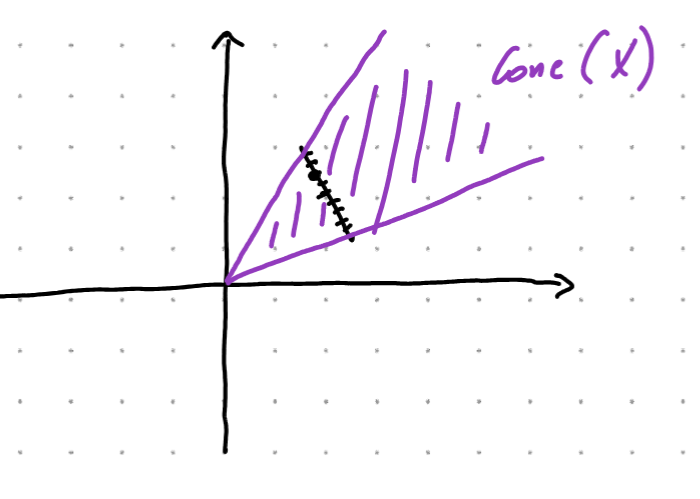
\includegraphics[width=0.7\textwidth]{img/cone.png}
    \caption{$X$ (black) and cone generated by $X$ (purple)}
\end{figure}

